\documentclass[14pt, oneside]{book}

% Packages
	\usepackage[margin=1in]{geometry}
	\usepackage{graphicx}
	\usepackage{svg}
		\svgpath{images/}
	\usepackage[font={small}]{caption}
	\usepackage{subcaption}
	\usepackage{wrapfig}
	\usepackage[bookmarks]{hyperref}
	\usepackage{minted}
	\usepackage[inline]{enumitem}
	\usepackage[utf8]{inputenc}
	\usepackage{csquotes}
	\usepackage{fancyhdr}
	\usepackage{booktabs}
	\usepackage{longtable}
	\usepackage{siunitx}
	% \usepackage{showframe}

% Header and Footer
	\pagestyle{fancy}
	\fancypagestyle{plain}{
		\fancyhf{}
		\fancyfoot[L]{HOGWARTS SCHOOL OF WITCHCRAFT AND WIZARDRY}
		\fancyfoot[R]{\textbf{\thepage}}
		\renewcommand{\footrulewidth}{0.5pt}
	}
	% title-only
	% \renewcommand{\sectionmark}[1]{\markright{SEC.\ #1}{}}
	% \renewcommand{\chaptermark}[1]{\markboth{CH.\ #1}{}}
	% number-only
	% \renewcommand{\sectionmark}[1]{\markright{SEC. \thesection}{}}
	% \renewcommand{\chaptermark}[1]{\markboth{CH.\ \thechapter}{}}
	% both
	\renewcommand{\sectionmark}[1]{\markright{SEC.\ \thesection\ #1}{}}
	\renewcommand{\chaptermark}[1]{\markboth{CH.\ \thechapter\ #1}{}}

	\fancyhead[L]{\rightmark}
	\fancyhead[R]{\leftmark}
	\fancyfoot[L]{HOGWARTS SCHOOL OF WITCHCRAFT AND WIZARDRY}
	\fancyfoot[C]{}
	\fancyfoot[R]{\textbf{\thepage}}
	\renewcommand{\headrulewidth}{0.5pt}
	\renewcommand{\footrulewidth}{0.5pt}


\title{\large The Big Bang}
\author{Tejas Sanap}

\begin{document}

\frontmatter
	\maketitle
	\tableofcontents
	\listoffigures

\mainmatter
	\chapter{What is the big bang?}
		\section{Introduction}
		The Big Bang theory is a cosmological model for the observable universe from the earliest known periods through its subsequent large-scale evolution\cite{2004biba.book.....S}. The model describes how the universe expanded from a very high-density and high-temperature state, and offers a comprehensive explanation for a broad range of phenomena, including the abundance of light elements, the cosmic microwave background (CMB), large-scale structure and Hubble's law (the farther away galaxies are, the faster they are moving away from Earth). If the observed conditions are extrapolated backwards in time using the known laws of physics, the prediction is that just before a period of very high density there was a singularity which is typically associated with the Big Bang. Current knowledge is insufficient to determine if the singularity was primordial.
		
		Georges Lemaître first noted in 1927 that an expanding universe could be traced back in time to an originating single point, calling his theory that of the "primeval atom". The scientific community was once divided between supporters of two different theories, the Big Bang and the steady state theory, but a wide range of empirical evidence has strongly favored the Big Bang which is now universally accepted\cite{kragh1999cosmology}. In 1929, from analysis of galactic redshifts, Edwin Hubble concluded that galaxies are drifting apart; this is important observational evidence for an expanding universe. In 1964, the cosmic microwave background radiation was discovered, which was crucial evidence in favor of the hot Big Bang model\cite{partridge20073k}, since that theory predicted the existence of background radiation throughout the universe before it was discovered.
		
			The known physical laws of nature can be used to calculate the characteristics of the universe in detail back in time to an initial state of extreme density and temperature. Detailed measurements of the expansion rate of the universe place the Big Bang at around 13.8 billion years ago, which is thus considered the age of the universe. After its initial expansion, the universe cooled sufficiently to allow the formation of subatomic particles, and later atoms. Giant clouds of these primordial elements (mostly hydrogen, with some helium and lithium) later coalesced through gravity, eventually forming early stars and galaxies, the descendants of which are visible today. Astronomers also observe the gravitational effects of dark matter surrounding galaxies. Most of the matter in the universe seems to be in the form of dark matter, and the Big Bang theory and various observations indicate that it is not conventional baryonic matter (atoms). It is still not known exactly what dark matter is. More recently, measurements of the redshifts of supernovae indicate that the expansion of the universe is accelerating, an observation attributed to dark energy's existence\cite{2003RvMP...75..559P}.
		
			\begin{figure}[h]
				\begin{subfigure}{0.5\textwidth}
					\includesvg[width=\textwidth]{cmbr.svg}
					\caption{CMBR Intensity}
				\end{subfigure}
				\begin{subfigure}{0.4\textwidth}
					\includesvg[width=\textwidth]{PowerSpectrumExt.svg}
					\caption{Power Spectrun}
				\end{subfigure}
				\caption{CMBR}
			\end{figure}
		
			% \begin{figure}[h]
			% 	\begin{subfigure}{0.5\textwidth}
			% 		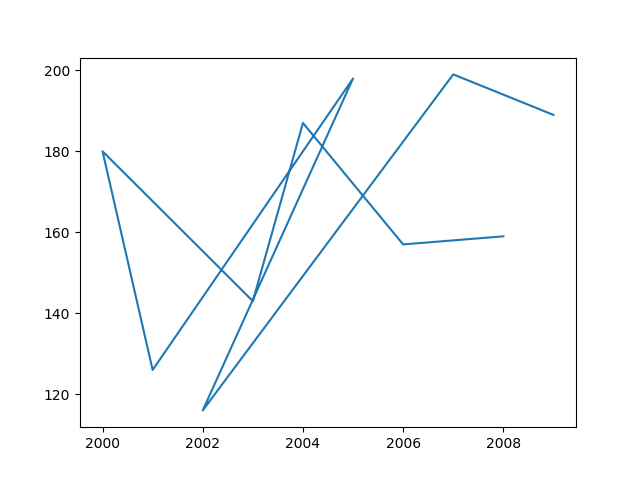
\includegraphics[width=\textwidth]{images/plot1.png}
			% 		\caption{\texttt{.png}}
			% 		\label{fig1}
			% 	\end{subfigure}
			% 	\begin{subfigure}{0.5\textwidth}
			% 		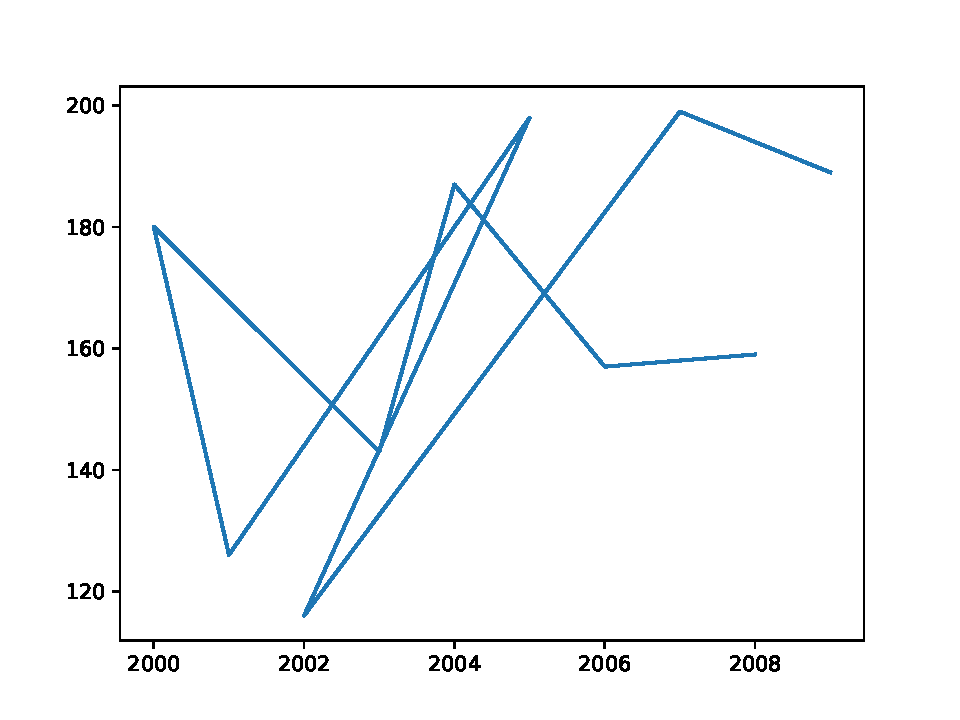
\includegraphics[width=\textwidth]{images/plot1.pdf}
			% 		\caption{$\texttt{.pdf}$}
			% 		\label{fig2}
			% 	\end{subfigure}
			% \end{figure}
	
		\section{Features of the Model}
			The Big Bang theory offers a comprehensive explanation for a broad range of observed phenomena, including the abundance of light elements, the CMB, large scale structure, and Hubble's Law. The Big Bang theory depends on two major assumptions: the universality of physical laws and the cosmological principle. The cosmological principle states that on large scales the universe is homogeneous and isotropic.
	
			These ideas were initially taken as postulates, but today there are efforts to test each of them. For example, the first assumption has been tested by observations showing that largest possible deviation of the fine structure constant over much of the age of the universe is of order 10---5. Also, general relativity has passed stringent tests on the scale of the Solar System and binary stars.
	
			If the large-scale universe appears isotropic as viewed from Earth, the cosmological principle can be derived from the simpler Copernican principle, which states that there is no preferred (or special) observer or vantage point. To this end, the cosmological principle has been confirmed to a level of 10---5 via observations of the CMB. The universe has been measured to be homogeneous on the largest scales at the 10% level.
	
			\subsection{Expansion of space}
				% \begin{figure}[h!]
				% 	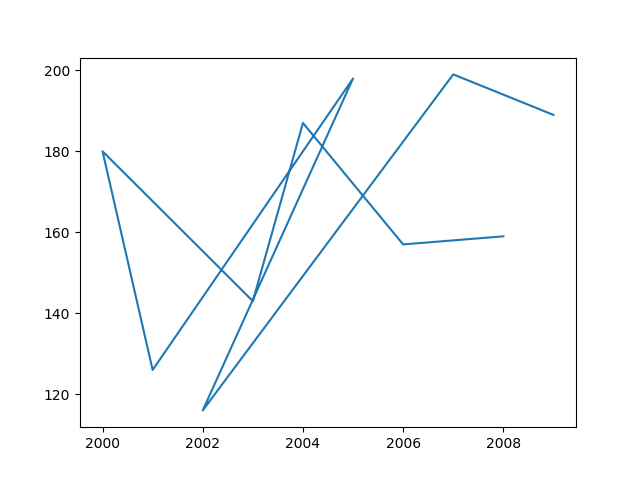
\includegraphics[width=0.5\textwidth]{images/plot1.png}
				% 	\caption{\texttt{.png}}
				% 	\label{fig1}
				% \end{figure}
				\begin{wrapfigure}{i}{0.5\textwidth}
					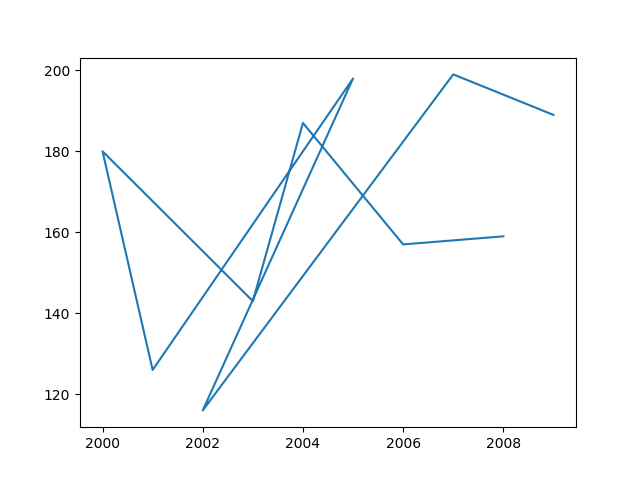
\includegraphics[width=\linewidth]{images/plot1.png}
					\caption{\texttt{.png}}
					\label{wrapfig:fig1}
				\end{wrapfigure}
	
				General relativity describes spacetime by a metric, which determines the distances that separate nearby points. The points, which can be galaxies, stars, or other objects, are themselves specified using a coordinate chart or "grid" that is laid down over all spacetime. The cosmological principle implies that the metric should be homogeneous and isotropic on large scales, which uniquely singles out the Friedmann–Lemaître–Robertson–Walker metric (FLRW metric). This metric contains a scale factor, which describes how the size of the universe changes with time. This enables a convenient choice of a coordinate system to be made, called comoving coordinates. In this coordinate system, the grid expands along with the universe, and objects that are moving only because of the expansion of the universe, remain at fixed points on the grid. While their coordinate distance (comoving distance) remains constant, the physical distance between two such co-moving points expands proportionally with the scale factor of the universe.
	
				The Big Bang is not an explosion of matter moving outward to fill an empty universe. Instead, space itself expands with time everywhere and increases the physical distance between two comoving points. In other words, the Big Bang is not an explosion in space, but rather an expansion of space. Because the FLRW metric assumes a uniform distribution of mass and energy, it applies to our universe only on large scales—local concentrations of matter such as our galaxy are gravitationally bound and as such do not experience the large-scale expansion of space.
	
			\subsection{Horizons}
				An important feature of the Big Bang spacetime is the presence of particle horizons. Since the universe has a finite age, and light travels at a finite speed, there may be events in the past whose light has not had time to reach us. This places a limit or a past horizon on the most distant objects that can be observed. Conversely, because space is expanding, and more distant objects are receding ever more quickly, light emitted by us today may never "catch up" to very distant objects. This defines a future horizon, which limits the events in the future that we will be able to influence. The presence of either type of horizon depends on the details of the FLRW model that describes our universe.
				\begin{wrapfigure}{i}{0.5\textwidth}
					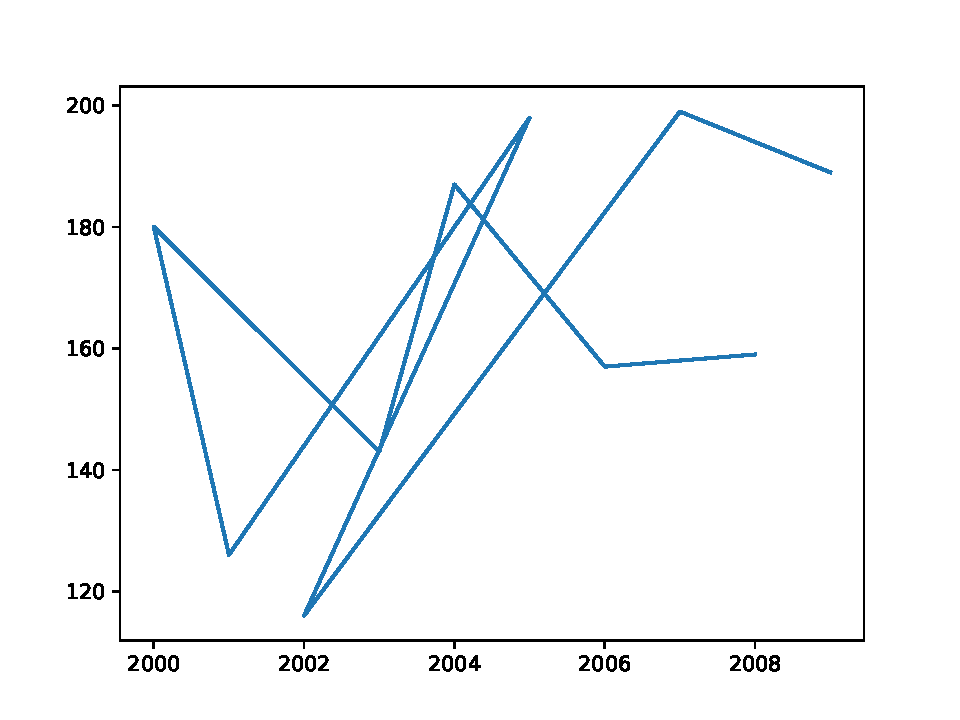
\includegraphics[width=\linewidth]{images/plot1.pdf}
					\caption{\texttt{.pdf}}
					\label{wrapfig:fig2}
				\end{wrapfigure}
				
				Our understanding of the universe back to very early times suggests that there is a past horizon, though in practice our view is also limited by the opacity of the universe at early times. So our view cannot extend further backward in time, though the horizon recedes in space. If the expansion of the universe continues to accelerate, there is a future horizon as well.

	\chapter{Timeline}
		\section{Singularity}
			Extrapolation of the expansion of the universe backwards in time using general relativity yields an infinite density and temperature at a finite time in the past. This singularity indicates that general relativity is not an adequate description of the laws of physics in this regime. Models based on general relativity alone can not extrapolate toward the singularity beyond the end of the Planck epoch.
			% match text within quote: /".\{-}"
			This primordial singularity is itself sometimes called ``the Big Bang", but the term can also refer to a more generic early hot, dense phase of the universe. In either case, ``the Big Bang" as an event is also colloquially referred to as the ``birth" of our universe since it represents the point in history where the universe can be verified to have entered into a regime where the laws of physics as we understand them (specifically general relativity and the standard model of particle physics) work. Based on measurements of the expansion using Type Ia supernovae and measurements of temperature fluctuations in the cosmic microwave background, the time that has passed since that event --- otherwise known as the ``age of the universe" --- is 13.799$\pm$0.021 billion years. The agreement of independent measurements of this age supports the $\Lambda$CDM model that describes in detail the characteristics of the universe.
			
			Despite being extremely dense at this time---far denser than is usually required to form a black hole---the universe did not re-collapse into a black hole. This may be explained by considering that commonly-used calculations and limits for gravitational collapse are usually based upon objects of relatively constant size, such as stars, and do not apply to rapidly expanding space such as the Big Bang.
		
		\section{Inflation and baryogenesis}
			The earliest phases of the Big Bang are subject to much speculation. In the most common models the universe was filled homogeneously and isotropically with a very high energy density and huge temperatures and pressures and was very rapidly expanding and cooling. Approximately 10--37 seconds into the expansion, a phase transition caused a cosmic inflation, during which the universe grew exponentially and during which time density fluctuations that occurred because of the uncertainty principle were amplified into the seeds that would later form the large-scale structure of the universe. After inflation stopped, reheating occurred until the universe obtained the temperatures required for the production of a quark–gluon plasma as well as all other elementary particles. Temperatures were so high that the random motions of particles were at relativistic speeds, and particle–antiparticle pairs of all kinds were being continuously created and destroyed in collisions. At some point, an unknown reaction called baryogenesis violated the conservation of baryon number, leading to a very small excess of quarks and leptons over antiquarks and antileptons---of the order of one part in 30 million. This resulted in the predominance of matter over antimatter in the present universe. 
		
		\goodbreak
		\section{Cooling}
			The universe continued to decrease in density and fall in temperature, hence the typical energy of each particle was decreasing. Symmetry breaking phase transitions put the fundamental forces of physics and the parameters of elementary particles into their present form. After about 10--11 seconds, the picture becomes less speculative, since particle energies drop to values that can be attained in particle accelerators. At about 10--6 seconds, quarks and gluons combined to form baryons such as protons and neutrons. The small excess of quarks over antiquarks led to a small excess of baryons over antibaryons. The temperature was now no longer high enough to create new proton–antiproton pairs (similarly for neutrons–antineutrons), so a mass annihilation immediately followed, leaving just one in 1010 of the original protons and neutrons, and none of their antiparticles. A similar process happened at about 1 second for electrons and positrons. After these annihilations, the remaining protons, neutrons and electrons were no longer moving relativistically and the energy density of the universe was dominated by photons (with a minor contribution from neutrinos).
	
			\begin{wrapfigure}{l}{0.4\textwidth}
				\centering
				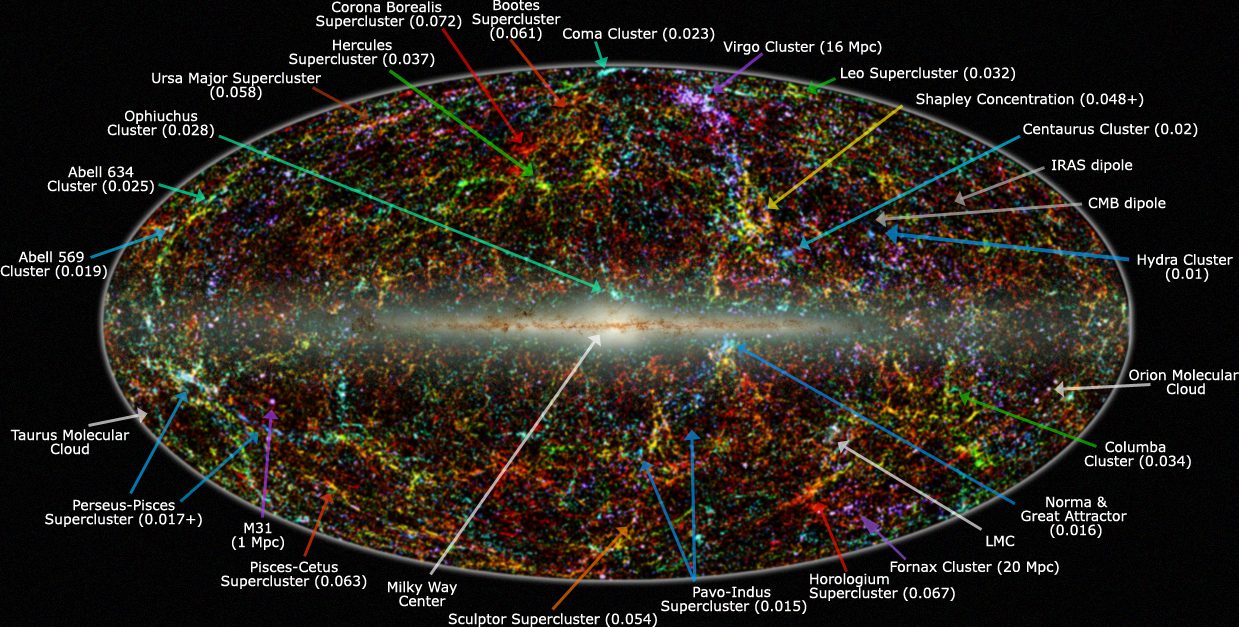
\includegraphics[width=0.9\linewidth]{images/near-infrared.jpg}
				\caption{Panoramic view of the entire near-infrared sky reveals the distribution of galaxies beyond the Milky Way. Galaxies are color-coded by redshift.}
				\label{img:redshift}
			\end{wrapfigure}
	
			A few minutes into the expansion, when the temperature was about a billion (one thousand million) kelvin and the density was about that of air, neutrons combined with protons to form the universe's deuterium and helium nuclei in a process called Big Bang nucleosynthesis. Most protons remained uncombined as hydrogen nuclei.
	
			As the universe cooled, the rest mass energy density of matter came to gravitationally dominate that of the photon radiation. After about 379,000 years, the electrons and nuclei combined into atoms (mostly hydrogen); hence the radiation decoupled from matter and continued through space largely unimpeded. This relic radiation is known as the cosmic microwave background radiation. The chemistry of life may have begun shortly after the Big Bang, 13.8 billion years ago, during a habitable epoch when the universe was only 10–17 million years old. 
	
		\section{Structure formation}
			Over a long period of time, the slightly denser regions of the nearly uniformly distributed matter gravitationally attracted nearby matter and thus grew even denser, forming gas clouds, stars, galaxies, and the other astronomical structures observable today. The details of this process depend on the amount and type of matter in the universe. The four possible types of matter are known as cold dark matter, warm dark matter, hot dark matter, and baryonic matter. The best measurements available, from Wilkinson Microwave Anisotropy Probe (WMAP), show that the data is well-fit by a Lambda-CDM model in which dark matter is assumed to be cold (warm dark matter is ruled out by early reionization), and is estimated to make up about 23\% of the matter/energy of the universe, while baryonic matter makes up about 4.6\%. In an "extended model" which includes hot dark matter in the form of neutrinos, then if the "physical baryon density" $\Omega_{b}h^{2}$ is estimated at about 0.023 (this is different from the 'baryon density' $\Omega_{b}$ expressed as a fraction of the total matter/energy density, which as noted above is about 0.046), and the corresponding cold dark matter density $\Omega_{c}h^{2}$ is about 0.11, the corresponding neutrino density $\Omega_{v}h^{2}$ is estimated to be less than 0.0062. 
	
		\section{Cosmic acceleration}
			Independent lines of evidence from Type Ia supernovae and the CMB imply that the universe today is dominated by a mysterious form of energy known as dark energy, which apparently permeates all of space. The observations suggest 73\% of the total energy density of today's universe is in this form. When the universe was very young, it was likely infused with dark energy, but with less space and everything closer together, gravity predominated, and it was slowly braking the expansion. But eventually, after numerous billion years of expansion, the growing abundance of dark energy caused the expansion of the universe to slowly begin to accelerate.
	
			Dark energy in its simplest formulation takes the form of the cosmological constant term in Einstein's field equations of general relativity, but its composition and mechanism are unknown and, more generally, the details of its equation of state and relationship with the Standard Model of particle physics continue to be investigated both through observation and theoretically.
	
			All of this cosmic evolution after the inflationary epoch can be rigorously described and modeled by the $\Lambda$CDM model of cosmology, which uses the independent frameworks of quantum mechanics and Einstein's General Relativity. There is no well-supported model describing the action prior to 10--15 seconds or so. Apparently a new unified theory of quantum gravitation is needed to break this barrier. Understanding this earliest of eras in the history of the universe is currently one of the greatest unsolved problems in physics.
	
	\chapter{History}
		\section{Etymology}
			English astronomer Fred Hoyle is credited with coining the term ``Big Bang" during a 1949 BBC radio broadcast, saying: ``These theories were based on the hypothesis that all the matter in the universe was created in one big bang at a particular time in the remote past."
			
			It is popularly reported that Hoyle, who favored an alternative ``steady state" cosmological model, intended this to be pejorative, but Hoyle explicitly denied this and said it was just a striking image meant to highlight the difference between the two models.
		
		\section{Development}
			The Big Bang theory developed from observations of the structure of the universe and from theoretical considerations. In 1912, Vesto Slipher measured the first Doppler shift of a ``spiral nebula" (spiral nebula is the obsolete term for spiral galaxies), and soon discovered that almost all such nebulae were receding from Earth. He did not grasp the cosmological implications of this fact, and indeed at the time it was highly controversial whether or not these nebulae were ``island universes" outside our Milky Way. Ten years later, Alexander Friedmann, a Russian cosmologist and mathematician, derived the Friedmann equations from Albert Einstein's equations of general relativity, showing that the universe might be expanding in contrast to the static universe model advocated by Einstein at that time. In 1924 Edwin Hubble's measurement of the great distance to the nearest spiral nebulae showed that these systems were indeed other galaxies. Independently deriving Friedmann's equations in 1927, Georges Lemaître, a Belgian physicist, proposed that the inferred recession of the nebulae was due to the expansion of the universe.
	
			In 1931 Lemaître went further and suggested that the evident expansion of the universe, if projected back in time, meant that the further in the past the smaller the universe was, until at some finite time in the past all the mass of the universe was concentrated into a single point, a ``primeval atom" where and when the fabric of time and space came into existence.
			
			Starting in 1924, Hubble painstakingly developed a series of distance indicators, the forerunner of the cosmic distance ladder, using the 100-inch (2.5 m) Hooker telescope at Mount Wilson Observatory. This allowed him to estimate distances to galaxies whose redshifts had already been measured, mostly by Slipher. In 1929 Hubble discovered a correlation between distance and recession velocity—now known as Hubble's law. Lemaître had already shown that this was expected, given the cosmological principle.
			
			In the 1920s and 1930s almost every major cosmologist preferred an eternal steady state universe, and several complained that the beginning of time implied by the Big Bang imported religious concepts into physics; this objection was later repeated by supporters of the steady state theory. This perception was enhanced by the fact that the originator of the Big Bang theory, Georges Lemaître, was a Roman Catholic priest. Arthur Eddington agreed with Aristotle that the universe did not have a beginning in time, viz., that matter is eternal. A beginning in time was ``repugnant" to him. Lemaître, however, thought that
			
			\blockquote{ If the world has begun with a single quantum, the notions of space and time would altogether fail to have any meaning at the beginning; they would only begin to have a sensible meaning when the original quantum had been divided into a sufficient number of quanta. If this suggestion is correct, the beginning of the world happened a little before the beginning of space and time. }
			
			During the 1930s other ideas were proposed as non-standard cosmologies to explain Hubble's observations, including the Milne model, the oscillatory universe (originally suggested by Friedmann, but advocated by Albert Einstein and Richard Tolman) and Fritz Zwicky's tired light hypothesis.
			
			After World War II, two distinct possibilities emerged. One was Fred Hoyle's steady state model, whereby new matter would be created as the universe seemed to expand. In this model the universe is roughly the same at any point in time. The other was Lemaître's Big Bang theory, advocated and developed by George Gamow, who introduced Big Bang nucleosynthesis (BBN) and whose associates, Ralph Alpher and Robert Herman, predicted the CMB. Ironically, it was Hoyle who coined the phrase that came to be applied to Lemaître's theory, referring to it as ``this big bang idea" during a BBC Radio broadcast in March 1949. For a while, support was split between these two theories. Eventually, the observational evidence, most notably from radio source counts, began to favor Big Bang over Steady State. The discovery and confirmation of the CMB in 1964 secured the Big Bang as the best theory of the origin and evolution of the universe. Much of the current work in cosmology includes understanding how galaxies form in the context of the Big Bang, understanding the physics of the universe at earlier and earlier times, and reconciling observations with the basic theory.
			
			In 1968 and 1970 Roger Penrose, Stephen Hawking, and George F. R. Ellis published papers where they showed that mathematical singularities were an inevitable initial condition of general relativistic models of the Big Bang. Then, from the 1970s to the 1990s, cosmologists worked on characterizing the features of the Big Bang universe and resolving outstanding problems. In 1981, Alan Guth made a breakthrough in theoretical work on resolving certain outstanding theoretical problems in the Big Bang theory with the introduction of an epoch of rapid expansion in the early universe he called ``inflation". Meanwhile, during these decades, two questions in observational cosmology that generated much discussion and disagreement were over the precise values of the Hubble Constant and the matter-density of the universe (before the discovery of dark energy, thought to be the key predictor for the eventual fate of the universe).
			
			In the mid-1990s, observations of certain globular clusters appeared to indicate that they were about 15 billion years old, which conflicted with most then-current estimates of the age of the universe (and indeed with the age measured today). This issue was later resolved when new computer simulations, which included the effects of mass loss due to stellar winds, indicated a much younger age for globular clusters. While there still remain some questions as to how accurately the ages of the clusters are measured, globular clusters are of interest to cosmology as some of the oldest objects in the universe.
			
			Significant progress in Big Bang cosmology has been made since the late 1990s as a result of advances in telescope technology as well as the analysis of data from satellites such as COBE, the Hubble Space Telescope and WMAP. Cosmologists now have fairly precise and accurate measurements of many of the parameters of the Big Bang model, and have made the unexpected discovery that the expansion of the universe appears to be accelerating.
	
	\chapter{Observational evidence}
		The earliest and most direct observational evidence of the validity of the theory are the expansion of the universe according to Hubble's law (as indicated by the redshifts of galaxies), discovery and measurement of the cosmic microwave background and the relative abundances of light elements produced by Big Bang nucleosynthesis. More recent evidence includes observations of galaxy formation and evolution, and the distribution of large-scale cosmic structures, These are sometimes called the ``four pillars" of the Big Bang theory.
		
		Precise modern models of the Big Bang appeal to various exotic physical phenomena that have not been observed in terrestrial laboratory experiments or incorporated into the Standard Model of particle physics. Of these features, dark matter is currently subjected to the most active laboratory investigations. Remaining issues include the cuspy halo problem and the dwarf galaxy problem of cold dark matter. Dark energy is also an area of intense interest for scientists, but it is not clear whether direct detection of dark energy will be possible. Inflation and baryogenesis remain more speculative features of current Big Bang models. Viable, quantitative explanations for such phenomena are still being sought. These are currently unsolved problems in physics.
	
		\section{Hubble's law and the expansion of space}
			Observations of distant galaxies and quasars show that these objects are redshifted: the light emitted from them has been shifted to longer wavelengths. This can be seen by taking a frequency spectrum of an object and matching the spectroscopic pattern of emission lines or absorption lines corresponding to atoms of the chemical elements interacting with the light. These redshifts are uniformly isotropic, distributed evenly among the observed objects in all directions. If the redshift is interpreted as a Doppler shift, the recessional velocity of the object can be calculated. For some galaxies, it is possible to estimate distances via the cosmic distance ladder. When the recessional velocities are plotted against these distances, a linear relationship known as Hubble's law is observed: $v=H_{0}D$ where,
	
			\begin{description}[align=right]
				\item[$v$] is the recessional velocity of the galaxy or other distant object,
				\item[$D$] is the comoving distance to the object, and
				\item[$H_{0}$] is Hubble's constant, measured to be $70.4^{+1.3}_{-1.4}$ km/s/Mpc by the WMAP probe.
			\end{description}
			
			Hubble's law has two possible explanations. Either we are at the center of an explosion of galaxies -- which is untenable under the assumption of the Copernican principle -- or the universe is uniformly expanding everywhere. This universal expansion was predicted from general relativity by Alexander Friedmann in 1922 and Georges Lemaître in 1927, well before Hubble made his 1929 analysis and observations, and it remains the cornerstone of the Big Bang theory as developed by Friedmann, Lemaître, Robertson, and Walker.
			
			The theory requires the relation $v=HD$ to hold at all times, where $D$ is the comoving distance, $v$ is the recessional velocity, and $v$, $H$, and $D$ vary as the universe expands (hence we write $H_{0}$ to denote the present-day Hubble ``constant"). For distances much smaller than the size of the observable universe, the Hubble redshift can be thought of as the Doppler shift corresponding to the recession velocity v. However, the redshift is not a true Doppler shift, but rather the result of the expansion of the universe between the time the light was emitted and the time that it was detected.
			
			That space is undergoing metric expansion is shown by direct observational evidence of the Cosmological principle and the Copernican principle, which together with Hubble's law have no other explanation. Astronomical redshifts are extremely isotropic and homogeneous, supporting the Cosmological principle that the universe looks the same in all directions, along with much other evidence. If the redshifts were the result of an explosion from a center distant from us, they would not be so similar in different directions.
			
			Measurements of the effects of the cosmic microwave background radiation on the dynamics of distant astrophysical systems in 2000 proved the Copernican principle, that, on a cosmological scale, the Earth is not in a central position. Radiation from the Big Bang was demonstrably warmer at earlier times throughout the universe. Uniform cooling of the CMB over billions of years is explainable only if the universe is experiencing a metric expansion, and excludes the possibility that we are near the unique center of an explosion.
	
		\section{Galactic evolution and distribution}
			\begin{figure}[h]
				\centering
				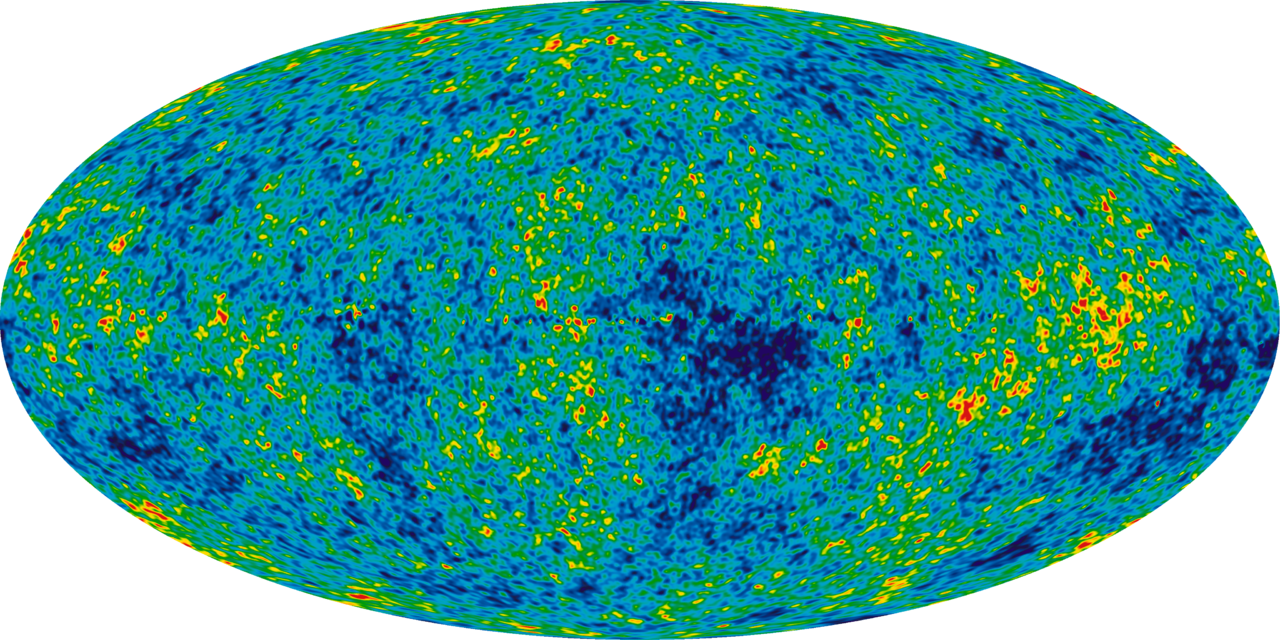
\includegraphics[width=0.7\textwidth, keepaspectratio]{images/cmbr.png}
				\caption{CMBR}
				\label{fig:cmbr}
			\end{figure}
			Detailed observations of the morphology and distribution of galaxies and quasars are in agreement with the current state of the Big Bang theory. A combination of observations and theory suggest that the first quasars and galaxies formed about a billion years after the Big Bang, and since then, larger structures have been forming, such as galaxy clusters and superclusters.
	
			Populations of stars have been aging and evolving, so that distant galaxies (which are observed as they were in the early universe) appear very different from nearby galaxies (observed in a more recent state). Moreover, galaxies that formed relatively recently, appear markedly different from galaxies formed at similar distances but shortly after the Big Bang. These observations are strong arguments against the steady-state model. Observations of star formation, galaxy and quasar distributions and larger structures, agree well with Big Bang simulations of the formation of structure in the universe, and are helping to complete details of the theory.
			
		\section{Primordial gas clouds}
			In 2011, astronomers found what they believe to be pristine clouds of primordial gas by analyzing absorption lines in the spectra of distant quasars. Before this discovery, all other astronomical objects have been observed to contain heavy elements that are formed in stars. These two clouds of gas contain no elements heavier than hydrogen and deuterium. Since the clouds of gas have no heavy elements, they likely formed in the first few minutes after the Big Bang, during Big Bang nucleosynthesis.
			
		\section{Other lines of evidence}
			The age of the universe as estimated from the Hubble expansion and the CMB is now in good agreement with other estimates using the ages of the oldest stars, both as measured by applying the theory of stellar evolution to globular clusters and through radiometric dating of individual Population II stars.
			
			The prediction that the CMB temperature was higher in the past has been experimentally supported by observations of very low temperature absorption lines in gas clouds at high redshift. This prediction also implies that the amplitude of the Sunyaev–Zel'dovich effect in clusters of galaxies does not depend directly on redshift. Observations have found this to be roughly true, but this effect depends on cluster properties that do change with cosmic time, making precise measurements difficult.
			
		\section{Future observations}
			Future gravitational waves observatories might be able to detect primordial gravitational waves, relics of the early universe, up to less than a second after the Big Bang. 
	
	\chapter{Steam Tables}
		% \setlength\LTleft{-0.5in}
		% \begin{longtable}{SSSSSSSSSSS}
\begin{longtable}{ccccccccccc}
\toprule
\textbf{P} & \textbf{T} & $v_{sl}$ & $v_{sg}$ & $IE_{g}$ & $IE_{l}$ & $H_l$ & vaporization & $H_g$ & $S_l$ & $S_g$ \\
\midrule
\endhead
0.00611  & 0.01        & 0.0010002              & 206.136             & 0                      & 2375.3              & 0.01            & 2501.3       & 2501.4       & 0              & 9.1562      \\
0.00813  & 4           & 0.0010001              & 157.232             & 16.77                  & 2380.9              & 16.78           & 2491.9       & 2508.7       & 0.061          & 9.0514      \\
0.00872  & 5           & 0.0010001              & 147.12              & 20.97                  & 2382.3              & 20.98           & 2489.6       & 2510.6       & 0.0761         & 9.0257      \\
0.00935  & 6           & 0.0010001              & 137.734             & 25.19                  & 2383.6              & 25.2            & 2487.2       & 2512.4       & 0.0912         & 9.0003      \\
0.01072  & 8           & 0.0010002              & 120.917             & 33.59                  & 2386.4              & 33.6            & 2482.5       & 2516.1       & 0.1212         & 8.9501      \\
0.01228  & 10          & 0.0010004              & 106.379             & 42                     & 2389.2              & 42.01           & 2477.7       & 2519.8       & 0.151          & 8.9008      \\
0.01312  & 11          & 0.0010004              & 99.857              & 46.2                   & 2390.5              & 46.2            & 2475.4       & 2521.6       & 0.1658         & 8.8765      \\
0.01402  & 12          & 0.0010005              & 93.784              & 50.41                  & 2391.9              & 50.41           & 2473         & 2523.4       & 0.1806         & 8.8524      \\
0.01497  & 13          & 0.0010007              & 88.124              & 54.6                   & 2393.3              & 54.6            & 2470.7       & 2525.3       & 0.1953         & 8.8285      \\
0.01598  & 14          & 0.0010008              & 82.848              & 58.79                  & 2394.7              & 58.8            & 2468.3       & 2527.1       & 0.2099         & 8.8048      \\
0.01705  & 15          & 0.0010009              & 77.926              & 62.99                  & 2396.1              & 62.99           & 2465.9       & 2528.9       & 0.2245         & 8.7814      \\
0.01818  & 16          & 0.0010011              & 73.333              & 67.18                  & 2397.4              & 67.19           & 2463.6       & 2530.8       & 0.239          & 8.7582      \\
0.01938  & 17          & 0.0010012              & 69.044              & 71.38                  & 2398.8              & 71.38           & 2461.2       & 2532.6       & 0.2535         & 8.7351      \\
0.02064  & 18          & 0.0010014              & 65.038              & 75.57                  & 2400.2              & 75.58           & 2458.8       & 2534.4       & 0.2679         & 8.7123      \\
0.02198  & 19          & 0.0010016              & 61.293              & 79.76                  & 2401.6              & 79.77           & 2456.5       & 2536.2       & 0.2823         & 8.6897      \\
0.02339  & 20          & 0.0010018              & 57.791              & 83.95                  & 2402.9              & 83.96           & 2454.1       & 2538.1       & 0.2966         & 8.6672      \\
0.02487  & 21          & 0.001002               & 54.514              & 88.14                  & 2404.3              & 88.14           & 2451.8       & 2539.9       & 0.3109         & 8.645       \\
0.02645  & 22          & 0.0010022              & 51.447              & 92.32                  & 2405.7              & 92.33           & 2449.4       & 2541.7       & 0.3251         & 8.6229      \\
0.0281   & 23          & 0.0010024              & 48.574              & 96.51                  & 2407                & 96.52           & 2447         & 2543.5       & 0.3393         & 8.6011      \\
0.02985  & 24          & 0.0010027              & 45.883              & 100.7                  & 2408.4              & 100.7           & 2444.7       & 2545.4       & 0.3534         & 8.5794      \\
0.03169  & 25          & 0.0010029              & 43.36               & 104.88                 & 2409.8              & 104.89          & 2442.3       & 2547.2       & 0.3674         & 8.558       \\
0.03363  & 26          & 0.0010032              & 40.994              & 109.06                 & 2411.1              & 109.07          & 2439.9       & 2549         & 0.3814         & 8.5367      \\
0.03567  & 27          & 0.0010035              & 38.774              & 113.25                 & 2412.5              & 113.25          & 2437.6       & 2550.8       & 0.3954         & 8.5156      \\
0.03782  & 28          & 0.0010037              & 36.69               & 117.42                 & 2413.9              & 117.43          & 2435.2       & 2552.6       & 0.4093         & 8.4946      \\
0.04     & 28.96       & 0.001004               & 34.8                & 121.45                 & 2415.2              & 121.46          & 2432.9       & 2554.4       & 0.4226         & 8.4746      \\
0.04008  & 29          & 0.001004               & 34.733              & 121.6                  & 2415.2              & 121.61          & 2432.8       & 2554.5       & 0.4231         & 8.4739      \\
0.04246  & 30          & 0.0010043              & 32.894              & 125.78                 & 2416.6              & 125.79          & 2430.5       & 2556.3       & 0.4369         & 8.4533      \\
0.04496  & 31          & 0.0010046              & 31.165              & 129.96                 & 2418                & 129.97          & 2428.1       & 2558.1       & 0.4507         & 8.4329      \\
0.04759  & 32          & 0.001005               & 29.54               & 134.14                 & 2419.3              & 134.15          & 2425.7       & 2559.9       & 0.4644         & 8.4127      \\
0.05034  & 33          & 0.0010053              & 28.011              & 138.32                 & 2420.7              & 138.33          & 2423.4       & 2561.7       & 0.4781         & 8.3927      \\
0.05324  & 34          & 0.0010056              & 26.571              & 142.5                  & 2422                & 142.5           & 2421         & 2563.5       & 0.4917         & 8.3728      \\
0.05628  & 35          & 0.001006               & 25.216              & 146.67                 & 2423.4              & 146.68          & 2418.6       & 2565.3       & 0.5053         & 8.3531      \\
0.05947  & 36          & 0.0010063              & 23.94               & 150.85                 & 2424.7              & 150.86          & 2416.2       & 2567.1       & 0.5188         & 8.3336      \\
0.06     & 36.16       & 0.0010064              & 23.739              & 151.53                 & 2425                & 151.53          & 2415.9       & 2567.4       & 0.521          & 8.3304      \\
0.06632  & 38          & 0.0010071              & 21.602              & 159.2                  & 2427.4              & 159.21          & 2411.5       & 2570.7       & 0.5458         & 8.295       \\
0.07384  & 40          & 0.0010078              & 19.523              & 167.56                 & 2430.1              & 167.57          & 2406.7       & 2574.3       & 0.5725         & 8.257       \\
0.08     & 41.51       & 0.0010084              & 18.103              & 173.87                 & 2432.2              & 173.88          & 2403.1       & 2577         & 0.5926         & 8.2287      \\
0.09593  & 45          & 0.0010099              & 15.258              & 188.44                 & 2436.8              & 188.45          & 2394.8       & 2583.2       & 0.6387         & 8.1648      \\
0.1      & 45.81       & 0.0010102              & 14.674              & 191.82                 & 2437.9              & 191.83          & 2392.8       & 2584.7       & 0.6493         & 8.1502      \\
0.1235   & 50          & 0.0010121              & 12.032              & 209.32                 & 2443.5              & 209.33          & 2382.7       & 2592.1       & 0.7038         & 8.0763      \\
0.1576   & 55          & 0.0010146              & 9.568               & 230.21                 & 2450.1              & 230.23          & 2370.7       & 2600.9       & 0.7679         & 7.9913      \\
0.1994   & 60          & 0.0010172              & 7.671               & 251.11                 & 2456.6              & 251.13          & 2358.5       & 2609.6       & 0.8312         & 7.9096      \\
0.2      & 60.06       & 0.0010172              & 7.649               & 251.38                 & 2456.7              & 251.4           & 2358.3       & 2609.7       & 0.832          & 7.9085      \\
0.2503   & 65          & 0.0010199              & 6.197               & 272.02                 & 2463.1              & 272.06          & 2346.2       & 2618.3       & 0.8935         & 7.831       \\
0.3      & 69.1        & 0.0010223              & 5.229               & 289.2                  & 2468.4              & 289.23          & 2336.1       & 2625.3       & 0.9439         & 7.7686      \\
0.3119   & 70          & 0.0010228              & 5.042               & 292.95                 & 2469.6              & 292.98          & 2333.8       & 2626.8       & 0.9549         & 7.7553      \\
0.3858   & 75          & 0.0010259              & 4.131               & 313.9                  & 2475.9              & 313.93          & 2321.4       & 2635.3       & 1.0155         & 7.6824      \\
0.4      & 75.87       & 0.0010265              & 3.993               & 317.53                 & 2477                & 317.58          & 2319.2       & 2636.8       & 1.0259         & 7.67        \\
0.4739   & 80          & 0.0010291              & 3.407               & 334.86                 & 2482.2              & 334.91          & 2308.8       & 2643.7       & 1.0753         & 7.6122      \\
0.5      & 81.33       & 0.00103                & 3.24                & 340.44                 & 2483.9              & 340.49          & 2305.4       & 2645.9       & 1.091          & 7.5939      \\
0.5783   & 85          & 0.0010325              & 2.828               & 355.84                 & 2488.4              & 355.9           & 2296         & 2651.9       & 1.1343         & 7.5445      \\
0.6      & 85.94       & 0.0010331              & 2.732               & 359.79                 & 2489.6              & 359.86          & 2293.6       & 2653.5       & 1.1453         & 7.532       \\
0.7      & 89.95       & 0.001036               & 2.365               & 376.63                 & 2494.5              & 376.7           & 2283.3       & 2660         & 1.1919         & 7.4797      \\
0.7014   & 90          & 0.001036               & 2.361               & 376.85                 & 2494.5              & 376.92          & 2283.2       & 2660.1       & 1.1925         & 7.4791      \\
0.8      & 93.5        & 0.001038               & 2.087               & 391.58                 & 2498.8              & 391.66          & 2274.1       & 2665.8       & 1.2329         & 7.4346      \\
0.8455   & 95          & 0.0010397              & 1.982               & 397.88                 & 2500.6              & 397.96          & 2270.2       & 2668.1       & 1.25           & 7.4159      \\
0.9      & 96.71       & 0.001041               & 1.869               & 405.06                 & 2502.6              & 405.15          & 2265.7       & 2670.9       & 1.2695         & 7.3949      \\
1        & 99.63       & 0.0010432              & 1.694               & 417.36                 & 2506.1              & 417.46          & 2258         & 2675.5       & 1.3026         & 7.3594      \\
1.014    & 100         & 0.0010435              & 1.673               & 418.94                 & 2506.5              & 419.04          & 2257         & 2676.1       & 1.3069         & 7.3549      \\
1.433    & 110         & 0.0010516              & 1.21                & 461.14                 & 2518.1              & 461.3           & 2230.2       & 2691.5       & 1.4185         & 7.2387      \\
1.5      & 111.4       & 0.0010528              & 1.159               & 466.94                 & 2519.7              & 467.11          & 2226.5       & 2693.6       & 1.4336         & 7.2233      \\
1.985    & 120         & 0.0010603              & 0.8919              & 503.5                  & 2529.3              & 503.71          & 2202.6       & 2706.3       & 1.5276         & 7.1296      \\
2        & 120.2       & 0.0010605              & 0.8857              & 504.49                 & 2529.5              & 504.7           & 2201.9       & 2706.7       & 1.5301         & 7.1271      \\
2.5      & 127.4       & 0.0010672              & 0.7187              & 535.1                  & 2537.2              & 535.37          & 2181.5       & 2716.9       & 1.6072         & 7.0527      \\
2.701    & 130         & 0.0010697              & 0.6685              & 546.02                 & 2539.9              & 546.31          & 2174.2       & 2720.5       & 1.6344         & 7.0269      \\
3        & 133.6       & 0.0010732              & 0.6058              & 561.15                 & 2543.6              & 561.47          & 2163.8       & 2725.3       & 1.6718         & 6.9919      \\
3.5      & 138.9       & 0.0010786              & 0.5243              & 583.95                 & 2546.9              & 584.33          & 2148.1       & 2732.4       & 1.7275         & 6.9405      \\
3.613    & 140         & 0.0010797              & 0.5089              & 588.74                 & 2550                & 589.13          & 2144.7       & 2733.9       & 1.7391         & 6.9299      \\
4        & 143.6       & 0.0010836              & 0.4625              & 604.31                 & 2553.6              & 604.74          & 2133.8       & 2738.6       & 1.7766         & 6.8959      \\
4.5      & 147.9       & 0.0010882              & 0.414               & 622.25                 & 2557.6              & 623.25          & 2120.7       & 2743.9       & 1.8207         & 6.8565      \\
4.758    & 150         & 0.0010905              & 0.3928              & 631.68                 & 2559.5              & 632.2           & 2114.3       & 2746.5       & 1.8418         & 6.8379      \\
5        & 151.9       & 0.0010926              & 0.3749              & 639.68                 & 2561.2              & 640.23          & 2108.5       & 2748.7       & 1.8607         & 6.8212      \\
6        & 158.9       & 0.0011006              & 0.3157              & 669.9                  & 2567.4              & 670.56          & 2086.3       & 2756.8       & 1.9312         & 6.76        \\
6.178    & 160         & 0.001102               & 0.3071              & 674.86                 & 2568.4              & 675.55          & 2082.6       & 2758.1       & 1.9427         & 6.7502      \\
7        & 165         & 0.001108               & 0.2729              & 696.44                 & 2572.5              & 697.22          & 2066.3       & 2763.5       & 1.9922         & 6.708       \\
7.917    & 170         & 0.0011143              & 0.2428              & 718.33                 & 2576.5              & 719.21          & 2049.5       & 2768.7       & 2.0419         & 6.6663      \\
8        & 170.4       & 0.0011148              & 0.2404              & 720.22                 & 2576.8              & 721.11          & 2048         & 2769.1       & 2.0462         & 6.6628      \\
9        & 175.4       & 0.0011212              & 0.215               & 741.83                 & 2580.5              & 742.83          & 2031.1       & 2773.9       & 2.0946         & 6.6226      \\
10       & 179.9       & 0.0011273              & 0.1944              & 761.68                 & 2583.6              & 762.81          & 2015.3       & 2778.1       & 2.1387         & 6.5863      \\
10.02    & 180         & 0.0011274              & 0.1941              & 762.09                 & 2583.7              & 763.22          & 2015         & 2778.2       & 2.1396         & 6.5857      \\
12.54    & 190         & 0.0011414              & 0.1565              & 806.19                 & 2590                & 807.62          & 1978.8       & 2786.4       & 2.2359         & 6.5079      \\
15       & 198.3       & 0.0011539              & 0.1318              & 843.16                 & 2594.5              & 844.84          & 1947.3       & 2792.2       & 2.315          & 6.4448      \\
15.54    & 200         & 0.0011565              & 0.1274              & 850.65                 & 2595.3              & 852.45          & 1940.7       & 2793.2       & 2.3309         & 6.4323      \\
19.06    & 210         & 0.0011726              & 0.1044              & 895.53                 & 2599.5              & 897.76          & 1900.7       & 2798.5       & 2.4248         & 6.3585      \\
20       & 212.4       & 0.0011767              & 0.09963             & 906.44                 & 2600.3              & 908.79          & 1890.7       & 2799.5       & 2.4474         & 6.3409      \\
23.18    & 220         & 0.00119                & 0.08619             & 940.87                 & 2602.4              & 943.62          & 1858.5       & 2802.1       & 2.5178         & 6.2861      \\
25       & 224         & 0.0011973              & 0.07998             & 959.11                 & 2603.1              & 962.11          & 1841         & 2803.1       & 2.5547         & 6.2575      \\
27.95    & 230         & 0.0012088              & 0.07158             & 986.74                 & 2603.9              & 990.12          & 1813.8       & 2804         & 2.6099         & 6.2146      \\
30       & 233.9       & 0.0012165              & 0.06668             & 1004.8                 & 2604.1              & 1008.4          & 1795.7       & 2804.2       & 2.6457         & 6.1869      \\
33.44    & 240         & 0.0012291              & 0.05976             & 1033.2                 & 2604                & 1037.3          & 1766.5       & 2803.8       & 2.7015         & 6.1437      \\
35       & 242.6       & 0.0012347              & 0.05707             & 1045.4                 & 2603.7              & 1049.8          & 1753.7       & 2803.4       & 2.7253         & 6.1253      \\
39.73    & 250         & 0.0012512              & 0.05013             & 1080.4                 & 2602.4              & 1085.4          & 1716.2       & 2801.5       & 2.7927         & 6.073       \\
40       & 250.4       & 0.0012522              & 0.04978             & 1082.3                 & 2602.3              & 1087.3          & 1714.1       & 2801.4       & 2.7964         & 6.0701      \\
45       & 257.5       & 0.0012692              & 0.04406             & 1116.2                 & 2600.1              & 1121.9          & 1676.4       & 2798.3       & 2.861          & 6.0199      \\
46.88    & 260         & 0.0012755              & 0.04221             & 1128.4                 & 2599                & 1134.4          & 1662.5       & 2796.6       & 2.8838         & 6.0019      \\
50       & 264         & 0.0012859              & 0.03944             & 1147.8                 & 2597.1              & 1154.2          & 1640.1       & 2794.3       & 2.9202         & 5.9734      \\
54.99    & 270         & 0.0013023              & 0.03564             & 1177.4                 & 2593.7              & 1184.5          & 1605.2       & 2789.7       & 2.9751         & 5.9301      \\
60       & 275.6       & 0.0013187              & 0.03244             & 1205.4                 & 2589.7              & 1213.4          & 1571         & 2784.3       & 3.0267         & 5.8892      \\
64.12    & 280         & 0.0013321              & 0.03017             & 1227.5                 & 2586.1              & 1236            & 1543.6       & 2779.6       & 3.0668         & 5.8571      \\
70       & 285.9       & 0.0013513              & 0.02737             & 1257.6                 & 2580.5              & 1267            & 1505.1       & 2772.1       & 3.1211         & 5.8133      \\
74.36    & 290         & 0.0013656              & 0.02557             & 1278.9                 & 2576                & 1289.1          & 1477.1       & 2766.2       & 3.1594         & 5.7821      \\
80       & 295.1       & 0.0013842              & 0.02352             & 1305.6                 & 2569.8              & 1316.6          & 1441.3       & 2758         & 3.2068         & 5.7432      \\
85.81    & 300         & 0.0014036              & 0.02167             & 1332                   & 2563                & 1344            & 1404.9       & 2749         & 3.2534         & 5.7045      \\
90       & 303.4       & 0.0014178              & 0.02048             & 1350.5                 & 2557.8              & 1363.3          & 1378.9       & 2742.1       & 3.2858         & 5.6772      \\
100      & 311.1       & 0.0014524              & 0.01803             & 1393                   & 2544.4              & 1407.6          & 1317.1       & 2724.7       & 3.3596         & 5.6141      \\
110      & 318.2       & 0.0014886              & 0.01599             & 1433.7                 & 2529.8              & 1450.1          & 1255.5       & 2705.6       & 3.4295         & 5.5527      \\
112.7    & 320         & 0.0014988              & 0.01549             & 1444.6                 & 2525.5              & 1461.5          & 1238.6       & 2700.1       & 3.448          & 5.5362      \\
120      & 324.8       & 0.0015267              & 0.01426             & 1473                   & 2513.7              & 1491.3          & 1193.6       & 2684.9       & 3.4962         & 5.4924      \\
130      & 330.9       & 0.0015671              & 0.01278             & 1511.1                 & 2496.1              & 1531.5          & 1130.7       & 2662.2       & 3.5606         & 5.4323      \\
140      & 336.8       & 0.0016107              & 0.01149             & 1548.6                 & 2476.8              & 1571.1          & 1066.5       & 2637.6       & 3.6232         & 5.3717      \\
145.9    & 340         & 0.0016379              & 0.0108              & 1570.3                 & 2464.6              & 1594.2          & 1027.9       & 2622         & 3.6594         & 5.3357      \\
150      & 342.2       & 0.0016581              & 0.01034             & 1585.6                 & 2455.5              & 1610.5          & 1000         & 2610.5       & 3.6848         & 5.3098      \\
160      & 347.4       & 0.0017107              & 0.009306            & 1622.7                 & 2431.7              & 1650.1          & 930.6        & 2580.6       & 3.7461         & 5.2455      \\
170      & 352.4       & 0.0017702              & 0.008364            & 1660.2                 & 2405                & 1690.3          & 856.9        & 2547.2       & 3.8079         & 5.1777      \\
180      & 357.1       & 0.0018397              & 0.007489            & 1698.9                 & 2374.3              & 1732            & 777.1        & 2509.1       & 3.8715         & 5.1044      \\
186.5    & 360         & 0.0018925              & 0.006945            & 1725.2                 & 2351.5              & 1760.5          & 720.5        & 2481         & 3.9147         & 5.0526      \\
190      & 361.5       & 0.0019243              & 0.006657            & 1739.9                 & 2338.1              & 1776.5          & 688          & 2464.5       & 3.9388         & 5.0228      \\
200      & 365.8       & 0.002036               & 0.005834            & 1785.6                 & 2293                & 1826.3          & 583.4        & 2409.7       & 4.0139         & 4.9269      \\
220.9    & 374.1       & 0.003155               & 0.003155            & 2029.6                 & 2029.6              & 2099.3          & 0            & 2099.3       & 4.4298         & 4.4298      \\
\bottomrule
\end{longtable}


	\bibliography{refs.bib}
	\bibliographystyle{alpha}

\end{document}
